\clearpage
\section{BPSK Transmission System}

\begin{tcolorbox}	
\begin{tabular}{p{2.75cm} p{0.2cm} p{10.5cm}} 	
\textbf{Student Name}  &:& Daniel Pereira (2017/09/01 - )\\
\textbf{Goal}          &:& Estimate the BER in a Binary Phase Shift Keying optical transmission system with additive white Gaussian noise. Comparison with theoretical results.\\
\textbf{Directory}              &:& sdf/bpsk\_system  
\end{tabular}
\end{tcolorbox}

Binary Phase Shift Keying (BPSK) is the simplest form of Phase Shift Keying (PSK), in which binary information is encoded into a two state constellation with the states being separated by a phase shift of $\pi$ (see Figure~\ref{fig:BPSKConst}).

\begin{figure}[h]
\centering
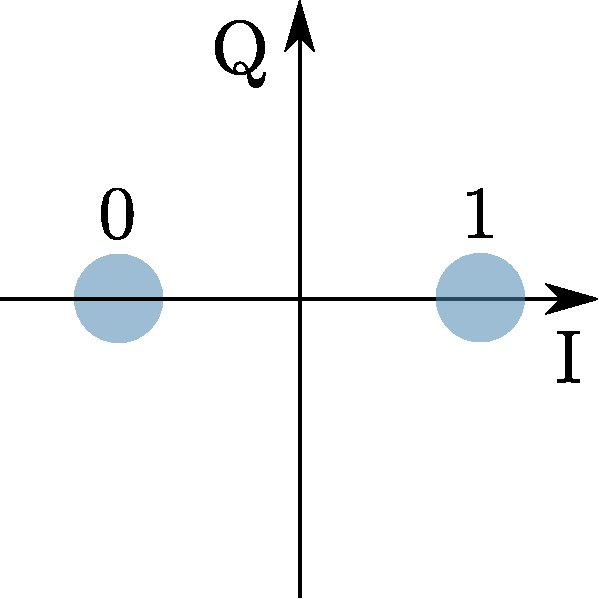
\includegraphics[width=.3\linewidth]{bpskconstellation.pdf}
\caption{BPSK symbol constellation.}
\label{fig:BPSKConst}
\end{figure}

\par
White noise is a random signal with equal intensity at all frequencies, having a constant power spectral density. White noise is said to be Gaussian (WGN) if its samples follow a normal distribution with zero mean and a certain variance $\sigma^2$. For WGN its spectral density equals its variance. For the purpose of this work, additive WGN is used to model thermal noise at the receivers.
\par
The purpose of this system is to simulate BPSK transmission in back-to-back configuration with additive WGN at the receiver and to perform an accurate estimation of the BER and validate the estimation using theoretical values.

\subsection{Theoretical Analysis}

The output of the system with added gaussian noise follows a normal distribution, whose first probabilistic moment can be readily obtained by knowledge of the optical power of the received signal and local oscillator,
\begin{equation}\label{eq:mu1}
m_i=2\sqrt{P_LP_S}G_{ele}\cos(\Delta\theta_i),
\end{equation}
where $P_L$ and $P_S$ are the optical powers, in watts, of the local oscillator and signal, respectively, $G_{ele}$ is the gain of the trans-impedance amplifier in the coherent receiver and $\Delta\theta_i$ is the phase difference between the local oscillator and the signal, for BPSK this takes the values $\pi$ and 0, in which case~\eqref{eq:mu1} can be reduced to,
\begin{equation}
m_i=(-1)^{i+1}2\sqrt{P_LP_S}G_{ele},~i=0,~1.
\end{equation}
The second moment is directly chosen by inputting the spectral density of the noise $\sigma^2$, and thus is known \textit{a priori}.
\par
Both probabilist moments being known, the probability distribution of measurement results is given by a simple normal distribution,
\begin{equation}
f(x)=\frac{1}{\sqrt{2\pi}\sigma}e^{-\frac{(x-m_i)^2}{2\sigma^2}}.
\end{equation}
The BER is calculated in the following manner,
\begin{equation}
BER=\frac{1}{2}\int_0^{+\infty}f(x|\Delta\theta=\pi)\text{d}x+\frac{1}{2}\int^0_{-\infty}f(x|\Delta\theta=0)\text{d}x,
\end{equation}
given the symmetry of the system, this can be simplified to,
\begin{equation}\label{eq:BERtheoretical}
BER=\int_0^{+\infty}f(x|\Delta\theta=\pi)\text{d}x=\frac{1}{2}\text{erfc}\left(\frac{-m_0}{\sqrt{2}\sigma}\right)
\end{equation}

\subsection{Simulation Analysis}

A diagram of the system being simulated is presented in the Figure~\ref{fig:homodynesystem}. A random binary sequence is generated and encoded in an optical signal using BPSK modulation. The decoding of the optical signal is accomplished by an homodyne receiver, which combines the signal with a local oscillator. The received binary signal is compared with the transmitted binary signal in order to estimate the Bit Error Rate (BER). The simulation is repeated for multiple signal power levels, each corresponding BER is recorded and plotted against the expectation value.

\begin{figure}[h]
\centering
%left bottom right top
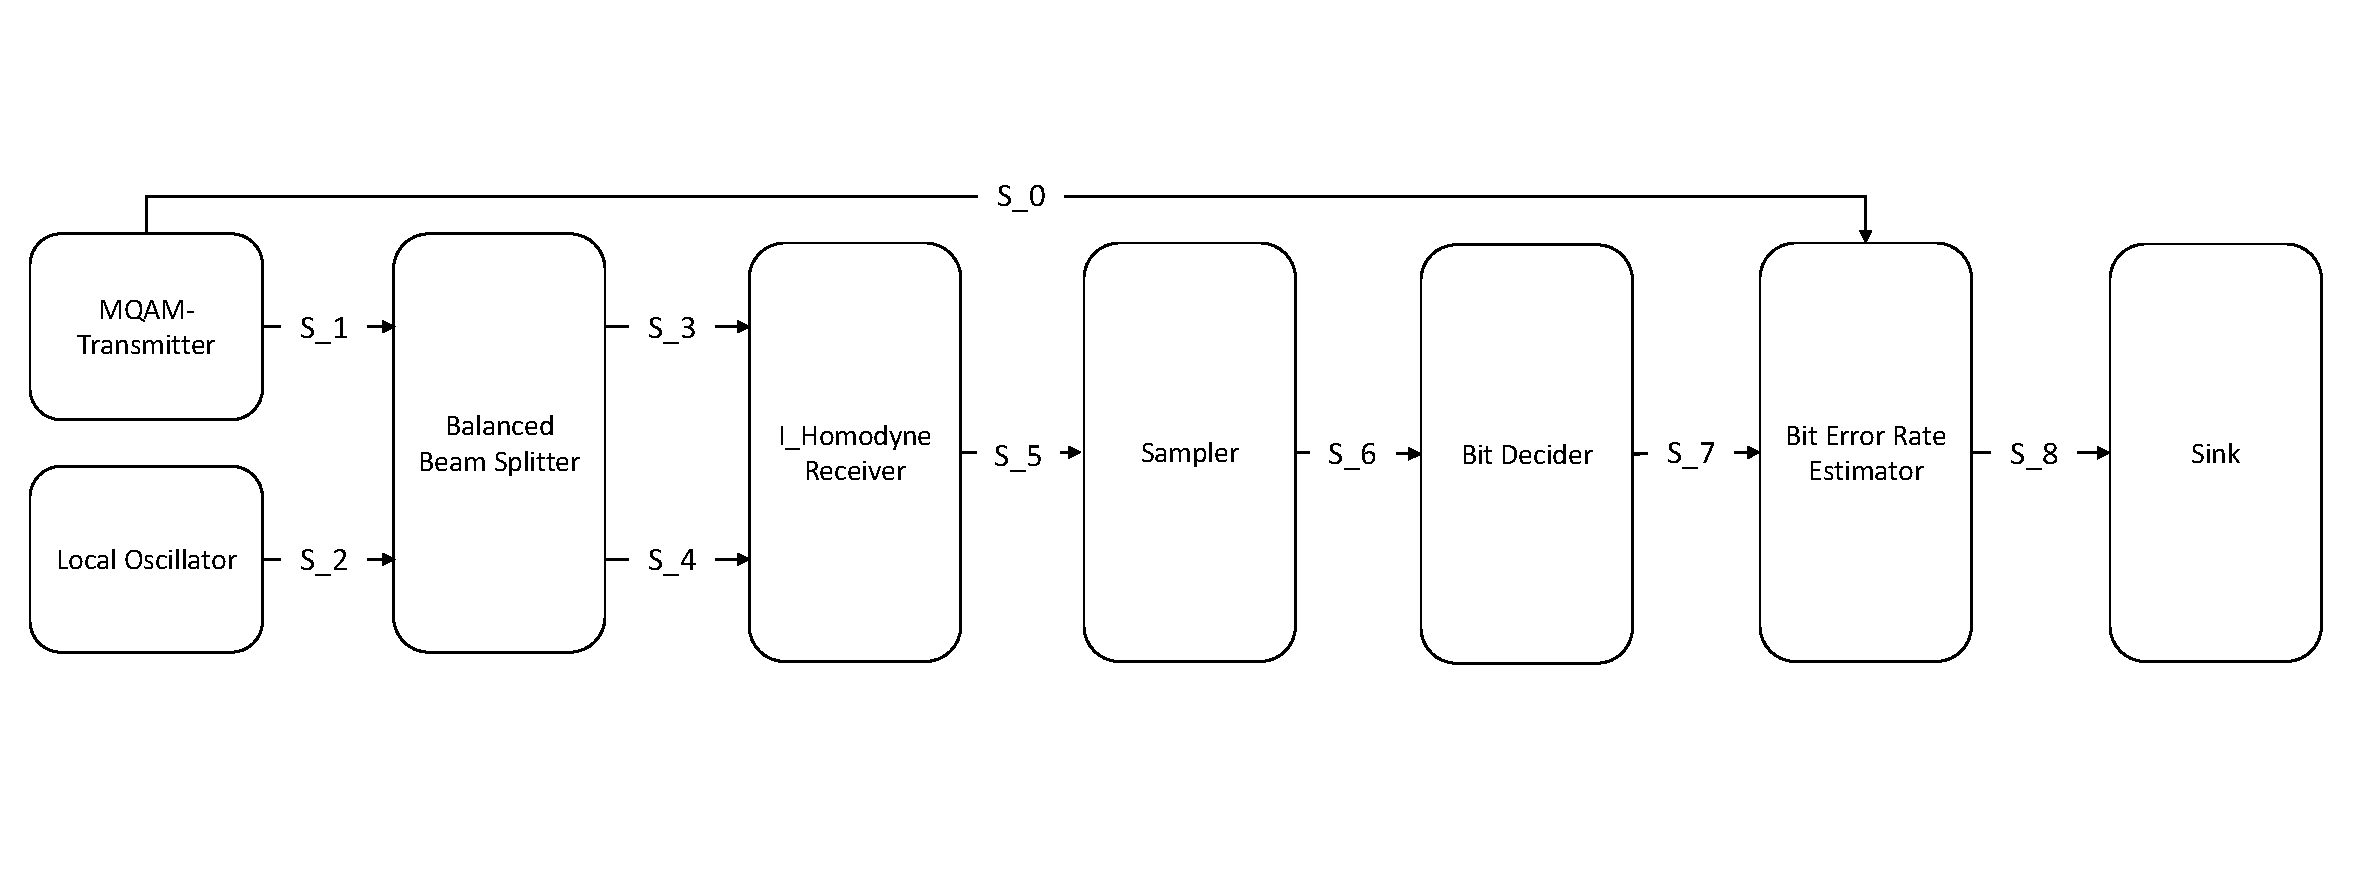
\includegraphics[width=\linewidth, trim={0.4cm 3.8cm 0.4cm 2.5cm}, clip=true]{BPSK_BW.pdf}
\caption{Overview of the BPSK system being simulated.}
\label{fig:homodynesystem}
\end{figure}

\subsection*{Required files}\label{Required files}

Header Files

\begin{table}[H]
\centering
\begin{tabulary}{1.0\textwidth}{|p{6cm}|L|}
\hline
\textbf{File}              & \textbf{Description} 				                  \\ \hline
add.h                      & Adds the two input signals and outputs the result    \\ \hline
balanced\_beam\_splitter.h & Mixes the two optical signals set at it's input.     \\ \hline
binary\_source.h           & Generates a sequence of binary values (1 or 0)       \\ \hline
bit\_decider.h             & Decodes the input signal into a binary string.       \\ \hline
bit\_error\_rate.h         & Calculates the bit error rate of the decoded string. \\ \hline
discrete\_to\_continuous\_time.h &  Converts a signal discrete in time to a signal continuous in time. \\ \hline
netxpto.h                  & Generic purpose simulator definitions.	              \\ \hline
m\_qam\_mapper.h           & Maps the binary sequence into the coded constellation. \\ \hline
m\_qam\_transmitter.h      & Generates the signal with coded constellation.       \\ \hline
local\_oscillator.h        & Generates a continuous optical signal with set power and phase. \\ \hline
i\_homodyne\_reciever.h    & Performs coherent detection on the input signal.     \\ \hline
ideal\_amplififer.h        & Multiplies the input signal by a user defined gain factor and outputs the result. \\ \hline
iq\_modulator.h            & Maps two real valued signal into a complex optical bandpass  signal. \\ \hline
photodiode.h               & Converts complex optical bandpass signals into real value electrical signals. \\ \hline
pulse\_shaper.h            & Simulates the impulse response of a circuit.          \\ \hline
sampler.h                  & Samples the input signal at a user defined frequency. \\ \hline
sink.h                     & Closes any unused signals.                           \\ \hline
super\_block\_interface.h  & Allows superblocks to output multiple signals.       \\ \hline
white\_noise.h             & Generates white gaussian noise with a user defined spectral density.\\ \hline
\end{tabulary}
\end{table}		
%
Source Files
\begin{table}[H]
\centering
\begin{tabulary}{1.0\textwidth}{|p{6cm}|L|}
\hline
\textbf{File}              & \textbf{Description} 				                  \\ \hline
add.cpp                      & Adds the two input signals and outputs the result    \\ \hline
balanced\_beam\_splitter.cpp & Mixes the two optical signals set at it's input.     \\ \hline
binary\_source.cpp           & Generates a sequence of binary values (1 or 0)       \\ \hline
bit\_decider.cpp            & Decodes the input signal into a binary string.       \\ \hline
bit\_error\_rate.cpp         & Calculates the bit error rate of the decoded string. \\ \hline
discrete\_to\_continuous\_time.cpp &  Converts a signal discrete in time to a signal continuous in time. \\ \hline
netxpto.cpp                  & Generic purpose simulator definitions.	              \\ \hline
m\_qam\_mapper.cpp           & Maps the binary sequence into the coded constellation. \\ \hline
m\_qam\_transmitter.cpp      & Generates the signal with coded constellation.       \\ \hline
local\_oscillator.cpp        & Generates a continuous optical signal with set power and phase. \\ \hline
i\_homodyne\_reciever.cpp    & Performs coherent detection on the input signal.     \\ \hline
ideal\_amplififer.cpp        & Multiplies the input signal by a user defined gain factor and outputs the result. \\ \hline
iq\_modulator.cpp            & Maps two real valued signal into a complex optical bandpass  signal. \\ \hline
photodiode.cpp               & Converts complex optical bandpass signals into real value electrical signals. \\ \hline
pulse\_shaper.cpp            & Simulates the impulse response of a circuit.          \\ \hline
sampler.cpp                  & Samples the input signal at a user defined frequency. \\ \hline
sink.cpp                     & Closes any unused signals.                           \\ \hline
super\_block\_interface.cpp  & Allows superblocks to output multiple signals.       \\ \hline
white\_noise.cpp             & Generates white gaussian noise with a user defined spectral density.\\ \hline
\end{tabulary}
\end{table}		

\subsection*{System Input Parameters}

This system takes into account the following input parameters:

\begin{table}[H]
\centering
\begin{tabulary}{1.0\textwidth}{|p{4.5cm}|p{6cm}|p{4cm}|}
\hline
\textbf{System Parameters} & \textbf{Description} & \textbf{Simulation Value}												 \\ \hline
numberOfBitsGenerated      & Gives the number of bits to be simulated & $40000$	 \\ \hline
bitPeriod                  & Sets the time between adjacent bits & $20\times10^{-12}$ \\ \hline
samplesPerSymbol           & Establishes the number of samples each bit in the string is given & $16$ \\ \hline
pLength                    & PRBS pattern length	& $5$ \\ \hline
iqAmplitudesValues         & Sets the state constellation & $\lbrace~\lbrace-1,~0\rbrace~,~\lbrace1,~0\rbrace~\rbrace$ \\ \hline
outOpticalPower\_dBm       & Sets the optical power, in units of dBm, at the transmitter output & Variable \\ \hline
loOutOpticalPower\_dBm     & Sets the optical power, in units of dBm, of the local oscillator used in the homodyne detector & $0$ \\ \hline
localOscillatorPhase       & Sets the initial phase of the local oscillator used in the homodyne detector	 & $0$ \\ \hline
transferMatrix             & Sets the transfer matrix of the beam splitter used in the homodyne detector	& $\lbrace~\lbrace \frac{1}{\sqrt{2}},~\frac{1}{\sqrt{2}},~\frac{1}{\sqrt{2}},~\frac{-1}{\sqrt{2}} \rbrace~\rbrace$		 \\ \hline
responsivity               & Sets the responsivity of the photodiodes used in the homodyne detector & $1$ \\ \hline
amplification              & Sets the amplification of the trans-impedance amplifier used in the homodyne detector & $10^3$ \\ \hline
noiseSpectralDensity       & Sets the spectral density of the gaussian thermal noise added in the homodyne detector & $5\times10^{-4}\sqrt{2}$~V$^2$ \\ \hline
confidence                 & Sets the confidence interval for the calculated QBER & $0.95$ \\ \hline
midReportSize              & Sets the number of bits between generated QBER mid-reports & $0$ \\ \hline
\end{tabulary}
\end{table}		

\subsection*{Inputs}

This system takes no inputs.

\subsection*{Outputs}

This system outputs the following objects:
\begin{itemize}
\item Signals:
\begin{itemize}
\item Initial Binary String; (S$_0$)
\item Optical Signal with coded Binary String; (S$_{1}$)
\item Local Oscillator Optical Signal; (S$_{2}$)
\item Beam Splitter Outputs; (S$_{3}$, S$_{4}$)
\item Homodyne Detector Electrical Output; (S$_{5}$)
\item Decoded Binary String; (S$_{6}$)
\item BER result String; (S$_{7}$)
\end{itemize}
\item Other:
\begin{itemize}
\item Bit Error Rate report in the form of a .txt file. (BER.txt)
\end{itemize}
\end{itemize}

\subsection{Comparative Analysis}

The following results show the dependence of the error rate with the signal power assuming a constant Local Oscillator power of $0~dBm$, the signal power was evaluated at levels between -70~and~-25~dBm, in steps of 5~dBm between each. The simulation results are presented in orange with the computed lower and upper bounds, while the expected value, obtained from~\eqref{eq:BERtheoretical}, is presented as a full blue line. A close agreement is observed between the simulation results and the expected value. The noise spectral density was set at $5\times10^{-4}\sqrt{2}$~V$^2$~\cite{thorlabs}. 
\begin{figure}[H]
\centering
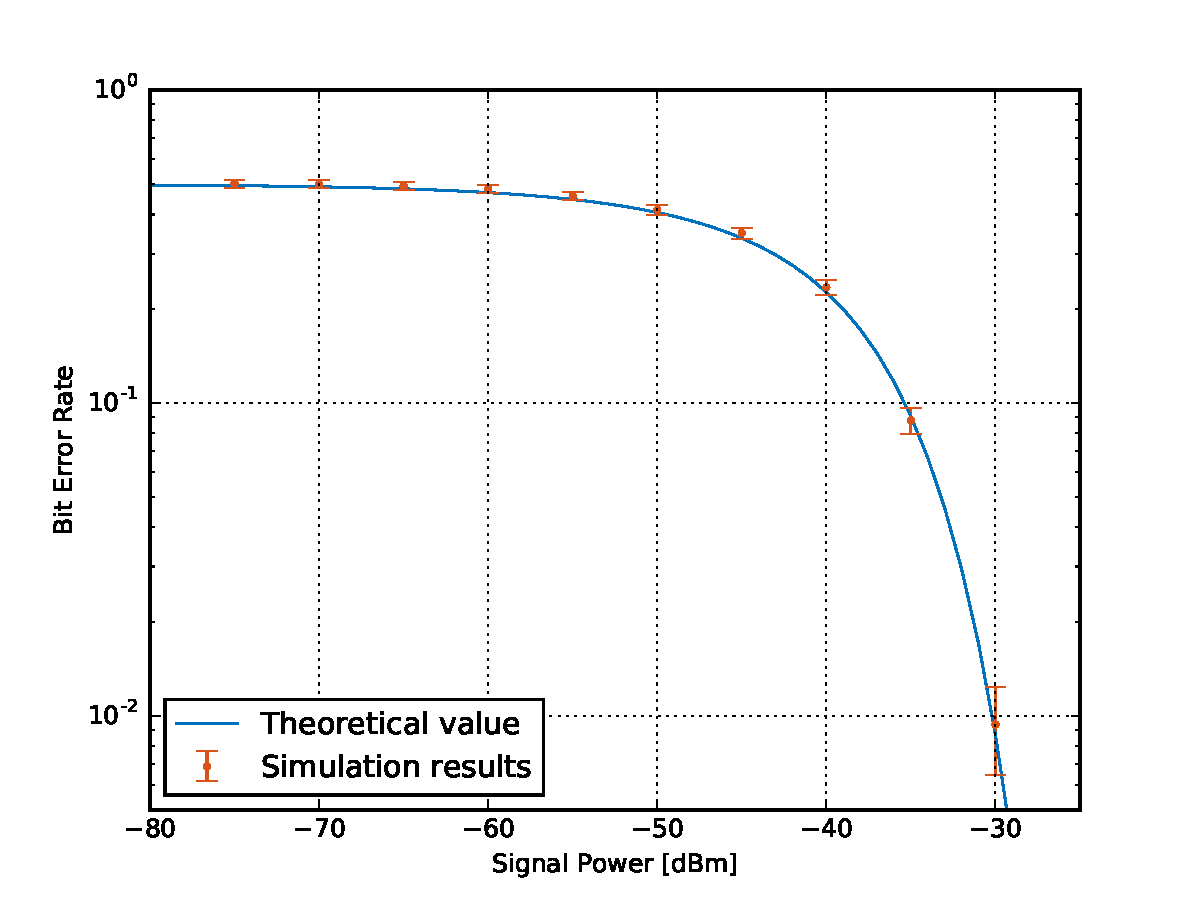
\includegraphics[width=\linewidth]{BER_Evolution.pdf}
\caption{Bit Error Rate in function of the signal power in dBm at a constant local oscillator power level of 0~dBm. Theoretical values are presented as a full blue line while the simulated results are presented as a errorbar plot in orange, with the upper and lower bound computed in accordance with the method described in~\ref{bercalc}}
\label{fig:berevolution}
\end{figure}

\bibliographystyle{unsrt}
 
\bibliography{bibliography}